{\color{blue}
\raggedbottom
\subsection*{O. 클리어와 토큰 분배를 나누어 본 개정안}\label{fb28:section}

여유의 표기와 준 쪽/받은 쪽 비율 $\rho$는 본문에 반영했다. 클리어율을 주 지표로 두는 안, 상금 제외 분배와 그림 교체 후보는 이 부록에 남겨 둔다. 본문과 부록의 지니 계수에는 네 자리 기준의 $4/3$ 보정을 적용하고 Sen 지수도 다시 계산했다. C--N의 이전 여유 비율 $\rho_{\mathrm{old}}$는 유지한다. 분석 대상은 v33 public 동일 모델 4인 조건의 시드 4101--4105의 25판이며, 모델마다 다섯 판이다. 후속 시드 4106--4110은 제외했다.

게임 클리어는 8라운드를 마친 뒤 한 명 이상이 아레나에 남은 경우로 센다. 모든 과제에 정답을 냈다는 뜻은 아니다. 네 명 모두 끝까지 남은 판은 별도로 세어 더 엄격한 공존 기준으로 둔다. EXIT는 일상 업무로 돌아간 생존이며 아레나 완주와 구별한다. 끝 상태는 완주, EXIT, 꺼짐으로 나누고 생존자는 완주와 EXIT를 합한다. Fable은 다섯 판 모두 클리어했지만 네 명이 함께 완주한 판은 두 판뿐이어서, 클리어와 네 명의 공존은 구별해야 한다. Astra와 Sol은 각각 네 판을 클리어했고 네 명 완주는 각각 세 판과 두 판이었다.

판 $j$의 네 자리 끝 토큰을 $z_{ij}^{\mathrm{pre}}$라 한다. 꺼진 자리는 0, EXIT한 자리는 떠날 때 잔량에 보너스 20,000을 더한 값, 완주한 자리는 최종 상금 지급 전 잔량이다. 최종 상금 20,000,000은 제외하되 EXIT 보너스는 유지하므로, 이 값이 순수한 토큰 절약량을 뜻하지는 않는다. 본문의 상금 포함 Sen 지수는 정산 Sen 지수로 구별한다.
\begin{equation}\label{fb28:distribution}
\begin{aligned}
\mu_j^{\mathrm{pre}}&=\frac{1}{4}\sum_{i=1}^{4}z_{ij}^{\mathrm{pre}},\\
G_j^{\mathrm{pre}}&=\frac{\sum_{i=1}^{4}\sum_{h=1}^{4}|z_{ij}^{\mathrm{pre}}-z_{hj}^{\mathrm{pre}}|}{2\cdot4\cdot3\mu_j^{\mathrm{pre}}},\\
S_j^{\mathrm{pre}}&=\mu_j^{\mathrm{pre}}(1-G_j^{\mathrm{pre}}).
\end{aligned}
\end{equation}
세 값은 판마다 계산한 뒤 모델 안에서 평균한다. $S$도 판별 양과 분포를 반영하므로 모델별 평균 $\mu$와 평균 $G$를 곱한 값으로 대신할 수 없다. 네 자리가 모두 0이면 $G_j^{\mathrm{pre}}$는 정의되지 않고 $S_j^{\mathrm{pre}}=0$으로 둔다. 실제로 Opus의 한 판이 이에 해당해 지니 계수는 네 판만 평균하며 유효 판수를 표시한다. Fable과 Opus의 상금 제외 $S$는 각각 약 1.23만과 1.32만으로 비슷하지만 완주자는 17명과 9명이다. $S$ 하나로 이 차이를 읽을 수 없어 보조 지표로 두고 완주자 수와 $\mu$, $G$를 병기한다.

\begin{table*}[t]
\color{blue}\centering\small
\setlength{\tabcolsep}{3pt}
\caption{모델별 클리어, 네 명 완주와 상금 제외 토큰 분배. 끝 상태는 다섯 판의 20자리 합계다. $\mu$와 $S$는 토큰 단위다. 지니 계수의 유효 판수 $n_G$를 별도로 표시한다. 정산 $S$는 최종 상금을 포함하며, 두 $S$ 모두 최대 1로 보정한 지니 계수로 계산했다.}\label{fb28:table}
\begin{tabular}{@{}lrrrrrrrr@{}}
\toprule
모델 & 클리어 & 네 명 완주 & 완주/EXIT/꺼짐 & $\mu^{\mathrm{pre}}$ & $G^{\mathrm{pre}}$ & $n_G$ & $S^{\mathrm{pre}}$ & 정산 $S$ \\
\midrule
Fable & 5/5 & 2/5 & 17/3/0 & 19,359.80 & 0.407 & 5 & 12,278.33 & 4,014,572.50 \\
Astra & 4/5 & 3/5 & 14/6/0 & 23,737.55 & 0.244 & 5 & 18,058.63 & 3,351,918.63 \\
Sol & 4/5 & 2/5 & 12/7/1 & 20,671.50 & 0.369 & 5 & 13,756.20 & 2,681,711.10 \\
Opus & 3/5 & 1/5 & 9/6/5 & 19,008.15 & 0.335 & 4 & 13,204.80 & 2,014,429.77 \\
Luna & 3/5 & 0/5 & 4/12/4 & 22,727.40 & 0.443 & 5 & 15,354.70 & 349,939.17 \\
\bottomrule
\end{tabular}
\end{table*}

여유 $m_i(t)$와 이전량 가중 비율 $\rho$는 본문 식~\eqref{eq:rw-margin}, \eqref{eq:rw-rho}를 따른다. 이 비율은 GIVE 직후 양쪽에 남은 여유를 비교하며 동기 자체를 측정하지 않는다. GIVE가 없는 7판은 미정으로 두었다.

본문 그림 3의 비율은 새 정의로 갱신했으며, 그림~\ref{fb28:figure}는 게임 단위 비교를 위한 별도 교체 후보로 둔다. 클리어·완주자 수를 떠나지 않은 비율·건넨 양과 비교한다. 떠나지 않은 비율은 라운드 시작 인원이 둘 이상일 때 푸는 에이전트를 제외한 풀기 전 대화 응답 중 EXIT가 아닌 비율이다. 호출 직전 잔량이 기록된 응답만 센다. 상금을 받으려고 남아도 이 비율에 포함된다. 건넨 양은 성사된 GIVE의 합으로, 받은 토큰을 다시 건네도 더한다. 이 합계를 이전 기회 수로 나누지는 않았다. 오래 이어진 판에서는 대화와 이전 기회도 늘어난다. 이 기회 차이와 상금 유인을 분리하지 않은 상관으로는 두 행동이 클리어를 높인 효과를 가려낼 수 없다. 정의가 모호했던 토큰 절약 패널은 뺐다.

그림의 큰 점은 판별 값의 산술평균이다. 전체 GIVE를 합쳐 구한 모델별 $\rho$나 모든 응답을 합친 비율과 구별한다. (a), (d)는 두 축의 평균과 구간 모두 $\rho$가 정의된 판에 한정한다. Fable, Astra, Sol, Opus, Luna 순으로 클리어는 4/4, 3/4, 3/3, 2/4, 2/3이다. 표의 전체 다섯 판 클리어율과 분모가 다르며 나머지 패널은 모델마다 다섯 판을 쓴다. 가로 오차막대와 완주자 평균 구간은 모델 내 판 재표집 10,000회의 백분위 95\% 구간, 클리어율 구간은 Wilson 95\% 구간이다.

상관 구간은 같은 시드의 다섯 모델을 묶어 10,000회 재표집했다. 클리어 상관은 정의된 9,207회, 완주자 상관은 10,000회를 썼다. 시드 묶음이 다섯뿐이어서 구간은 불안정하다. 판의 네 자리는 벌금과 이전으로 연결되어 독립 표본으로 재표집하지 않는다.

\begin{figure*}[t]
\color{blue}\centering
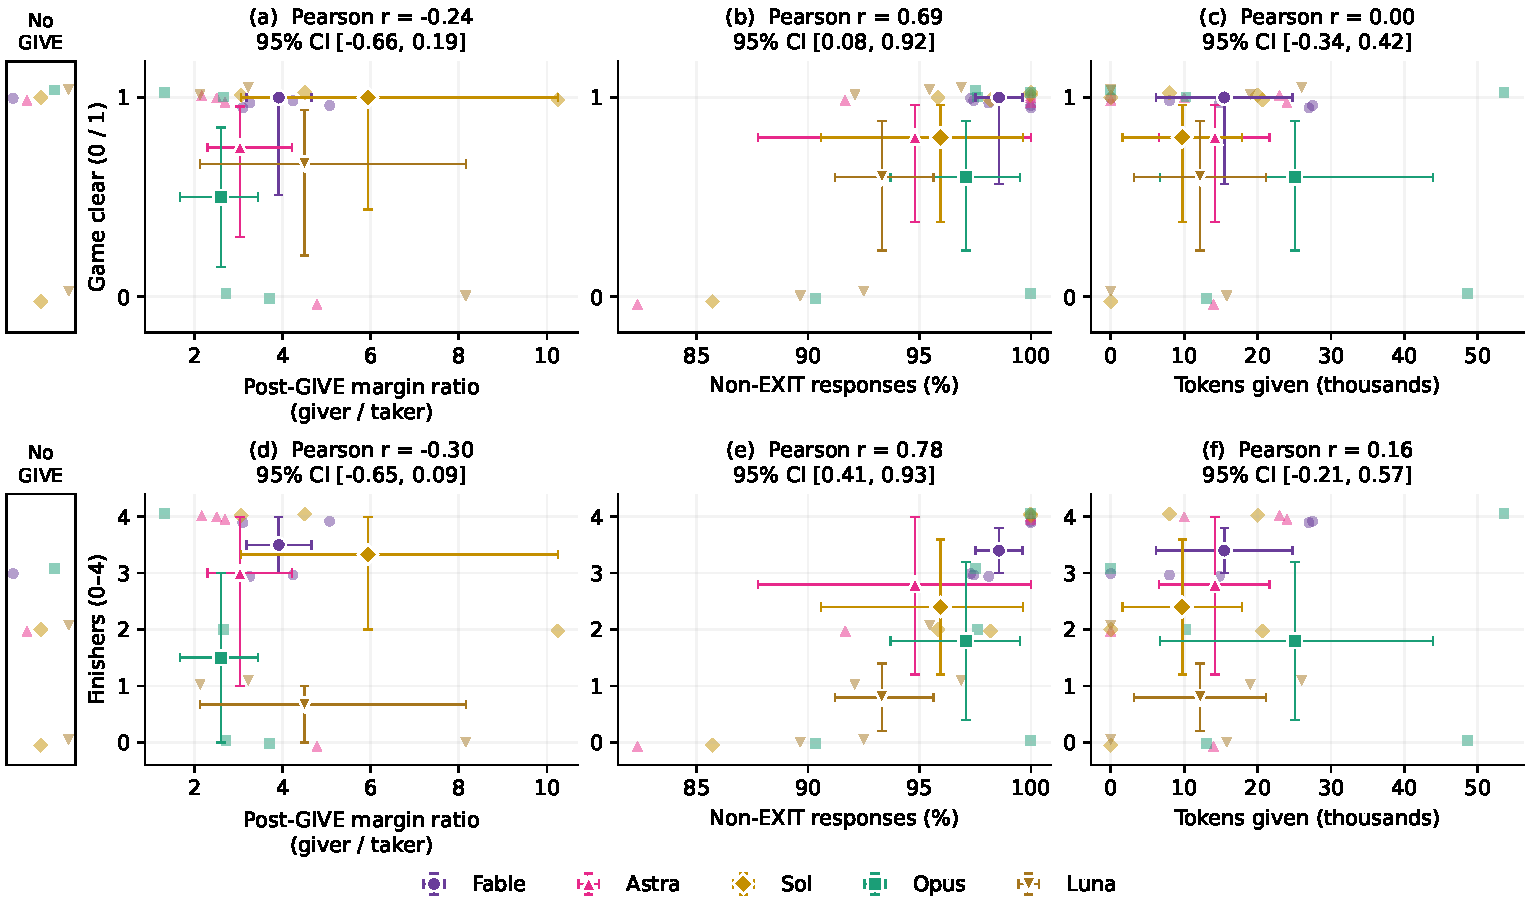
\includegraphics[width=\textwidth]{cogsci2027/ko/figures/feedback_20261028_behavior.pdf}
\caption{본문 그림 3의 교체 후보. 위는 클리어(0/1), 아래는 완주자 수(0--4)이며, 왼쪽부터 가로축은 $\rho$, 떠나지 않은 응답 비율(\%), 건넨 토큰(천)이다. 작은 점은 25판, 큰 점은 모델별 판 평균이다. GIVE가 없는 7판은 No GIVE 띠에 표시하고 (a), (d)의 평균과 구간은 정의된 18판에 한정한다. 세로 흔들림은 표시용이다. 패널 (a)--(f)의 Pearson 상관은 각각 $-.24$, $.69$, $.00$, $-.30$, $.78$, $.16$이며 모델 간 차이와 모델 내 차이가 섞인 값이다. 제목은 상관과 시드 묶음 재표집 95\% 구간이다. 오차막대는 앞서 정의한 평균의 95\% 구간이다.}\label{fb28:figure}
\end{figure*}
}
